\documentclass[11pt,a4paper]{article}
\usepackage[utf8]{inputenc}
\usepackage[T1]{fontenc}
\usepackage[spanish]{babel}
\usepackage{geometry}
\usepackage{graphicx}
\usepackage{booktabs}
\usepackage{float}
\geometry{margin=2.5cm}

\title{Informe técnico inicial: Fashion-MNIST}
\author{Ignacio Silva}
\date{16 de septiembre de 2026}

\begin{document}
\maketitle

\section{Propósito y alcance}
Este informe formal resume el bloque inicial del proyecto EP1: contrato de datos, exploración, preprocesamiento, baseline E0 y comparaciones iniciales de activación y pérdida. El informe complementa ---no reemplaza--- el registro operativo en \texttt{docs/collaborators/ignacio/REPORT.md}. El conjunto oficial de test no fue usado.

\section{Entorno reproducible}
El entorno local se creó con \texttt{uv venv --python 3.12 .venv}. La ejecución validada utilizó Python 3.12.14, TensorFlow 2.21.0, NumPy 2.5.3, Pandas 3.0.5 y scikit-learn 1.9.1; las versiones están bloqueadas en \texttt{uv.lock}. Se detectó CPU y ninguna GPU disponible en TensorFlow nativo de Windows; las pruebas funcionales y los experimentos se ejecutaron por CPU.

\section{Datos y preprocesamiento}
Fashion-MNIST contiene 60.000 imágenes oficiales de entrenamiento y 10.000 de test, con forma $28\times28$, tipo \texttt{uint8}, rango $[0,255]$ y diez clases balanceadas. El train oficial se dividió mediante índices estratificados, semilla 42 y fracción 10\%: 54.000 ejemplos de train y 6.000 de validation, con 5.400/600 ejemplos por clase. Las imágenes se convirtieron a \texttt{float32} y se normalizaron a $[0,1]$. Las etiquetas se codificaron one-hot para salida Softmax y categorical crossentropy.

\begin{figure}[H]
\centering
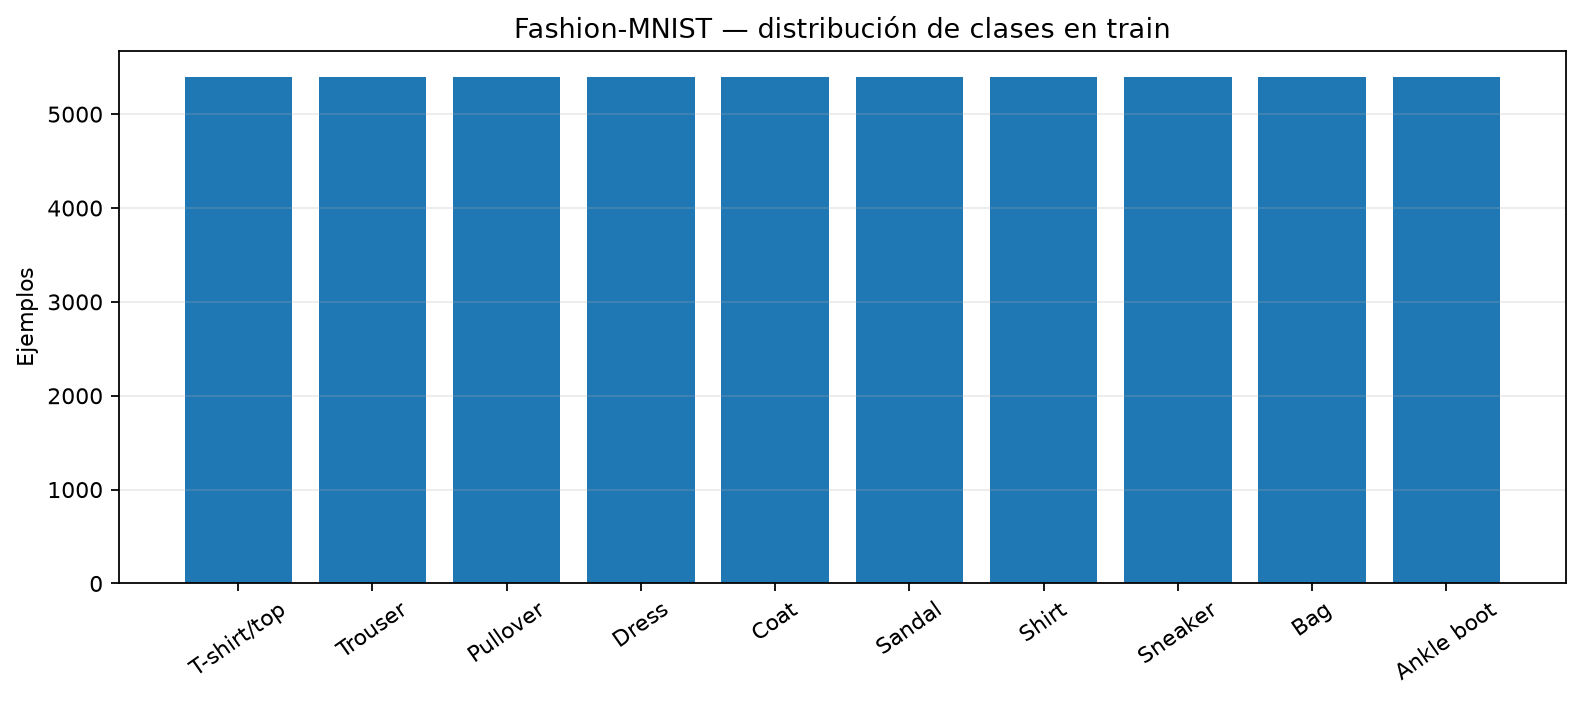
\includegraphics[width=0.9\linewidth]{../../../../results/figures/D0_train_class_distribution.png}
\caption{Distribución balanceada de clases en train.}
\end{figure}

\section{Baseline E0}
E0 usa una MLP con \texttt{Flatten}, capas Dense de 256 y 128 neuronas con ReLU, salida Softmax de diez unidades, categorical crossentropy, SGD con learning rate 0,01, batch size 128 y 20 épocas. No incorpora regularización. Tiene 235.146 parámetros.

\begin{table}[H]
\centering
\begin{tabular}{lr}
\toprule
Métrica de validation & Resultado \\
\midrule
Accuracy & 0,8722 \\
Precision ponderada & 0,8737 \\
Recall ponderado & 0,8722 \\
F1 ponderado & 0,8726 \\
\bottomrule
\end{tabular}
\caption{Resultados del baseline E0.}
\end{table}

La accuracy de validation aumentó de 0,7592 a 0,8722; la loss de validation bajó de 0,7395 a 0,3666. No se observó un gap claro de sobreajuste en esta corrida, por lo que L2 no se introdujo todavía.

\begin{figure}[H]
\centering
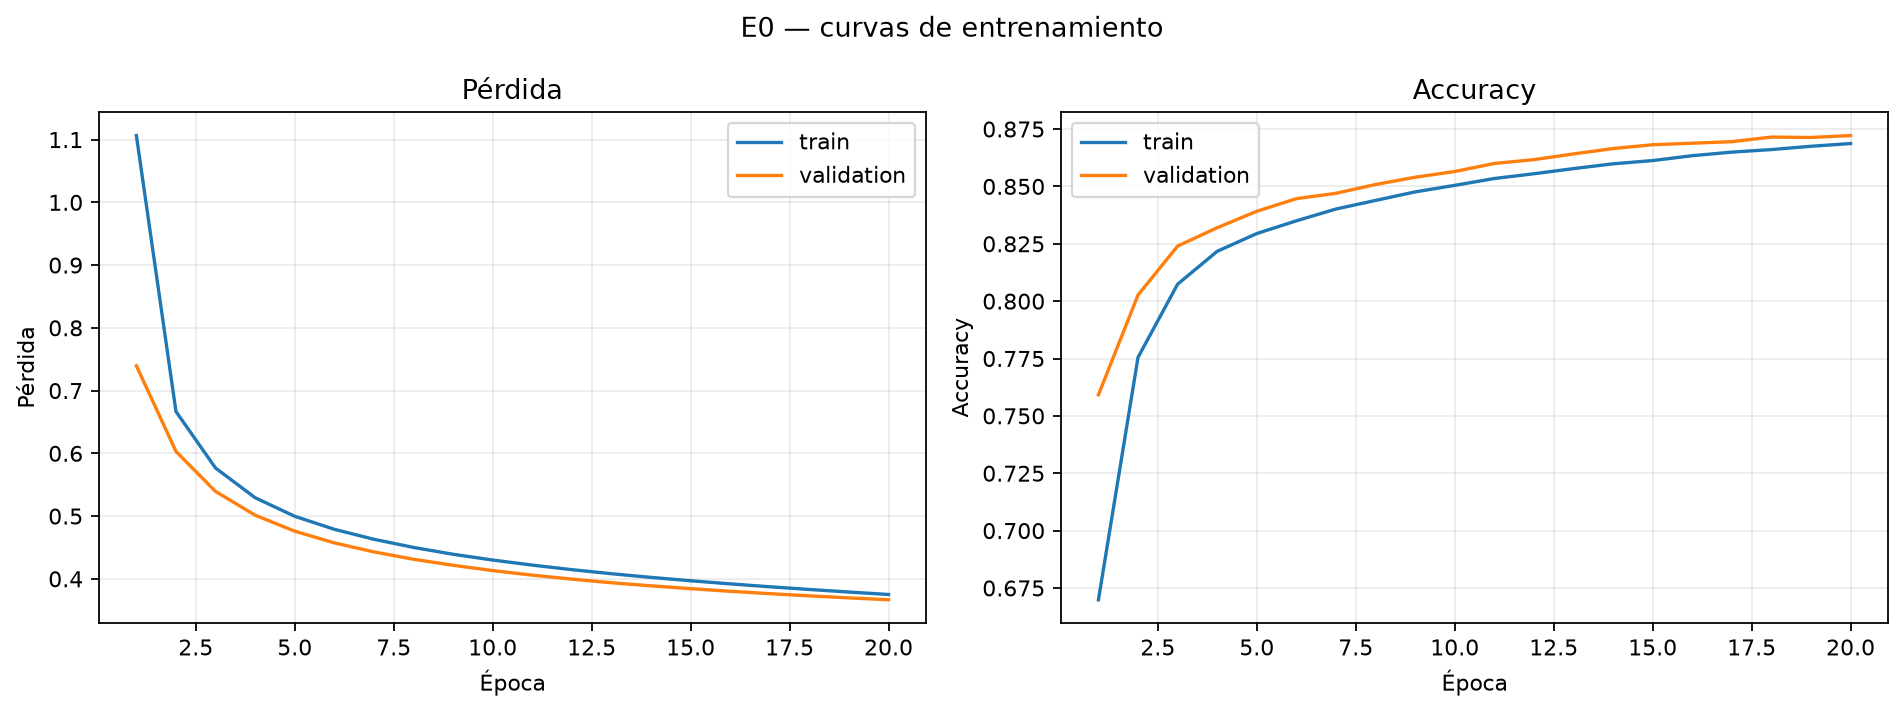
\includegraphics[width=\linewidth]{../../../../results/figures/E0_curves.png}
\caption{Curvas train/validation de E0.}
\end{figure}

\section{Comparaciones controladas}
Se mantuvieron fijas partición, seed, arquitectura, optimizador, learning rate, batch size y épocas. Solo se modificó una variable por ejecución.

\begin{table}[H]
\centering
\begin{tabular}{llrr}
\toprule
ID & Único cambio & Accuracy validation & F1 ponderado \\
\midrule
E0 & ReLU + categorical crossentropy & 0,8722 & 0,8726 \\
E1\_tanh & Tanh & 0,8643 & 0,8647 \\
E1\_sigmoid & Sigmoid & 0,7535 & 0,7490 \\
E2\_mse & MSE & 0,7370 & 0,7168 \\
\bottomrule
\end{tabular}
\caption{Comparación inicial sobre validation.}
\end{table}

ReLU y categorical crossentropy quedan seleccionados como control para la siguiente etapa. Esto no constituye una selección final y no habilita evaluación sobre test.

\section{Reproducción y handoff}
Las 12 pruebas automatizadas pasan dentro de \texttt{.venv}; incluyen contrato de datos, partición, normalización, construcción de E0, salida Softmax y coherencia de configuración. El notebook \texttt{notebooks/01\_ignacio\_data\_baseline.ipynb} ejecuta desde un kernel limpio. Lucas debe reutilizar E0 exclusivamente como control para estudiar learning rate, batch size, capacidad y Early Stopping; Cesar debe revisar este bloque antes de aceptarlo.

\end{document}
